
Suppose the quasi-linear equation admits the \textit{vacuum solution} $u \equiv 0$, i.e. the non-linearity satisfies $F(0) = 0$. If the non-linearity is continuously differentiable, then we can Taylor expand and reformulate the initial data problem as a \emph{semi-linear} equation, 
	\begin{equation}
		\begin{split}
			\partial_t u - Lu 
				&= N(u), \\
			u_{|t = 0}
				&= u_0,	
		\end{split}
		\tag{sLin}
		\label{eq:sLin}
	\end{equation}
where $L \in \operatorname{End} (\R^n)$ is a linear operator and $N: \R^n \to \R^n$ is a non-linear operator which vanishes faster than linearly at zero, i.e.
	\[ \lim_{|u| \to 0} \frac{|N(u)|}{|u|} = 0. \]	
	
\subsection{Linear theory}
The case $N = 0$ corresponds to the \emph{homogeneous linear} equation,
	\begin{equation}
		\begin{split}
			\partial_t u - Lu 
				&= 0, \\
			u_{|t = 0}
				&= u_0.
		\end{split}
		\tag{0Lin}
		\label{eq:0Lin}
	\end{equation}
The evolution of this equation is driven by the \emph{linear propagator} $e^{tL} \in \operatorname{End} (\R^n)$. Observe that the propagator satisfies the \textit{group law} $e^{tL} e^{sL} = e^{(t + s) L}$ and $e^{0L} = \operatorname{Id}$. Linearity of the propagator $e^{tL} (u_0 + v_0) = e^{tL} u_0 + e^{tL} v_0$ shows that the solutions to the homogeneous equation forms a vector space. This is known as the \emph{principle of superposition}.
	
\begin{theorem}[Linear propagators]
	Let $L : \R^n \to \R^n$ be linear, then the initial data problem for the homogeneous linear equation (\ref{eq:0Lin}) is globally well-posed and admits the solution formula
		\[ u(t) = e^{tL} u_0. \]
\end{theorem}

\begin{proof}
	In one-dimension $n = 1$, this can be derived from separation of variables. In arbitrary dimensions, we can multiply the equation by an integrating factor $e^{-tL}$, allowing us to rewrite it as $\partial_t (e^{-tL} u) = 0$. Applying the fundamental theorem of calculus furnishes the formula.
\end{proof}

\begin{remark}
	If $u_0 \in \R^n$ is an eigenvector of $L$, i.e. $Lu_0 = \lambda u_0$ for some $\lambda \in \C$, then the unique global solution is given by $u(t) = e^{t\lambda} u_0$. Thus, if all the eigenvalues of $L$ have negative real part, then the equation is \textit{dissipative}, decaying exponentially as $t\to + \infty$, and if all the eigenvalues have positive real part, then the equation is \textit{anti-dissipative}, growing exponentially as $t \to + \infty$. 
\end{remark}

Suppose now at every time $t$, the evolution of the linear equation is influenced by an external \textit{forcing term} $f \in C^0 (\R \to \R^n)$. This corresponds to the study of the \emph{inhomogeneous linear} equation
	\begin{equation}
		\begin{split}
			\partial_t u - Lu 
				&= f, \\
			u_{|t = 0}
				&= u_0.
		\end{split}
		\tag{fLin}
		\label{eq:fLin}
	\end{equation}
By linearity, we can solve the equation without loss of generality starting with zero initial data $u_0 = 0$. One can think of the inhomogeneous problem as a family of homogeneous problems at each time $t = t_0$ with initial data given by the infinitesimal force $f (s) ds$. Superimposing the corresponding solutions to each homogeneous problem furnishes the solution to the inhomogeneous problem. 

\begin{theorem}[Duhamel's formula]
	Let $L \in \operatorname{End} (\R^n)$ be a linear operator and $f \in C^0 (\R \to \R^n)$ be continuous. Then the initial data problem for the inhomogeneous linear equation (\ref{eq:fLin}) is globally well-posed and admits the solution formula
		\[ u(t) = e^{t L} u_0 + \int_0^t e^{(t - s) L} f(s) \, ds .\]	
\end{theorem}

\begin{proof}
	We use the method of integrating factors, making the ansatz $u(t) = e^{tL} v(t)$ for some $v \in C^1 (\R \to \R^n)$ such that $v(0) = u_0$. This allows us to write the inhomogeneous equation as 
		\[ \partial_t v = e^{tL} f. \]
	By the fundamental theorem of calculus, this is equivalent to 
		\[ v(t) = u_0 + \int_0^t e^{-s L} f(s) \, ds. \]
	Multiplying both sides by $e^{tL}$ and using the group law furnishes Duhamel's formula. 		
\end{proof}

\subsection{Duhamel iteration}

In view of Duhamel's formula, we see that solving the semi-linear problem (\ref{eq:sLin}) is equivalent to solving the integral equation 
	\begin{align}
		u(t) =  u_{\text{lin}} + DN u(t)
		\tag{sLin'} 
		\label{eq:abs}
	\end{align}	
where $u_{\text{lin}} \in C^0 ([0, T] \to \R^n)$ is the linear evolution of initial data and $D : C^0 ([0, T] \to \R^n) \to C^0 ([0, T] \to \R^n)$ is the Duhamel operator,
	\[ u_{\text{lin}} := e^{tL} u_0 ,\qquad DF (t) := \int_0^t e^{(t - s) L} F(s) \, ds. \]	
We will argue by \textit{Duhamel iteration}. Schematically, we start off with an approximate solution $u^{(0)} := u_{\text{lin}}$, and inductively construct subsequent approximates $u^{(n)}$ be inputting $u^{(n - 1)}$ into Duhamel's formula, 
	\[ u^{(n)} := u_{\text{lin}} + DN u^{(n - 1)}.  \]
These approximate solutions are known as \emph{Duhamel iterates}, and the goal then is to show that this sequence $\{u^{(n)}\}_n$ converges uniformly to some $u$. To this end, we modify the contraction mapping scheme.

	\begin{figure}[h]
		\begin{center}
			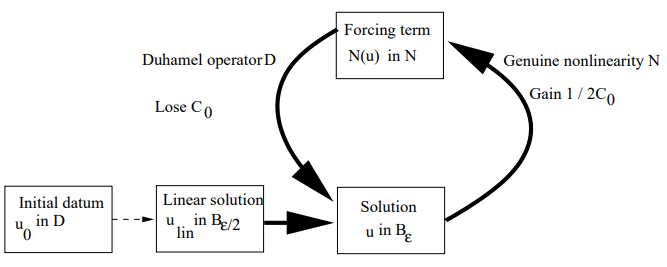
\includegraphics[scale = 0.8]{duhamel}
			\caption{The abstract Duhamel iteration scheme.}
		\end{center}
	\end{figure}

\begin{lemma}[Abstract Duhamel iteration]
	Let $\cN$ and $\cS$ be Banach spaces. Suppose  $D: \cN \to \cS$ is a bounded linear operator such that
		\[ ||DF||_{\cS} \leq C ||F||_{\cN}, \]
	and	 $N : \cS \to \cN$ is a Lipschitz non-linear operator such that $N(0) = 0$ and 
		\[ ||Nu - Nv||_{\cN} \leq \frac{1}{2C} ||u - v||_{\cS}, \]
	for all $u, v \in \overline{B_\epsilon (0)}$. Then for all $u_{\text{lin}} \in \overline{B_{\epsilon/2} (0)}$, there exists a unique solution $u \in \overline{B_\epsilon (0)}$ to the equation (\ref{eq:abs}), with the map $u_{\text{lin}} \mapsto u$ Lipschitz with constant at most $2$.
\end{lemma}

\begin{proof}
	Solving the equation (\ref{eq:abs}) is equivalent to finding a fixed point of the operator $\Phi : \cS \to \cS$ defined by 
		\[ \Phi (u) := u_{\text{lin}} + DNu. \]
	We claim this map is a contraction on the closed ball $\overline{B_\epsilon (0)} \subseteq \cS$ with Lipschitz constant $\tfrac12$; the contraction mapping principle completes the proof. To show $\Phi$ maps the ball into itself, observe by the triangle inequality
		\[ ||\Phi (u)||_\cS \leq ||u_{\text{lin}}||_\cS + ||DNu||_\cS \leq \epsilon \]
	for any $u \in \overline{B_\epsilon (0)}$. To show $\Phi$ is a contraction, for any $u, v \in \cS$, we can write $\Phi(u) - \Phi(v) = D(Nu - Nv)$. Taking norms, we obtain 
		\[ ||\Phi (u) - \Phi(v)||_\cS \leq C ||Nu - Nv||_\cN \leq  \frac12 ||u - v||_\cS,  \]
	as desired. Similarly, to show that the linear-to-nonlinear solution map is Lipschitz continuous, we use the equation and the triangle inequality to write
		\[ ||u - v||_\cS \leq ||u_{\text{lin}} - v_{\text{lin}}||_\cS + ||D(Nu - Nv)||_\cS \leq ||u_{\text{lin}} - v_{\text{lin}}||_\cS + \frac12||u - v||_\cS.  \]
	Rearranging shows that the Lipschitz constant is at most $2$. 	
\end{proof}

\begin{remark}
	One should think of the space $\cS$ as the \textit{solution space} and $\cN$ as the space where the non-linearity resides. Making a judicious choice of these spaces so that the iteration scheme converges is a central problem in the study of semi-linear partial differential equations for small data. 
\end{remark}

\begin{figure}[h]
	\begin{center}
		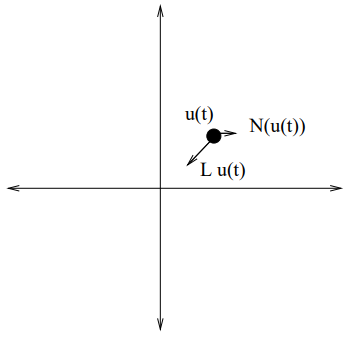
\includegraphics[scale = 0.7]{smalldata}
		\caption{For small data, the dissipative effect of the linear term $Lu$ dominates the non-linear term $Nu$, leading to global well-posedness and decay. }
	\end{center}
\end{figure}

\begin{theorem}[Linear stability implies non-linear stability]
	Let $L \in \operatorname{End} (\R^n)$ be a dissipative linear operator in that 
		\[ \langle Lu, u \rangle \leq - \sigma \langle u, u \rangle\]
	for some $\sigma > 0$, and suppose $N \in C^2_{\loc} (\R^n \to \R^n)$ vanishes faster than linearly at the origin. Then for initial data sufficiently close to the origin $|u_0| \ll 1$, there exists a unique global solution $u \in C^1 ([0, \infty) \to \R^n)$ to the semi-linear equation (\ref{eq:sLin}) obeying the exponential decay,
		\[ |u(t)| \leq 2 e^{-\sigma t} |u_0|. \]
\end{theorem}

\begin{proof}
	Define the solution space $\cS$ and the non-linearity space $\cN$ as subsets of the space of continuous functions $C^0 ([0, \infty) \to \R^n)$ such that the corresponding norms,
		\begin{align*}
			||u||_\cS
				&:= \sup_{t \geq 0} e^{\sigma t} |u(t)|, \\
			||u||_\cN
				&:= \sup_{t \geq 0} e^{\sigma t} |u(t)|
		\end{align*}
	are finite. By Gronwall's inequality, $||u_{\text{lin}}||_\cS \leq |u_0|$, so the triangle inequality implies
		\[ ||DF||_\cS \leq \frac1\sigma ||F||_\cN. \]
	Since $N$ vanishes super-linearly at the origin, Taylor expanding gives $|Nu - Nv| \ll |u - v| (|u| + |v|)$ for all $|u|, |v| \ll 1$. In particular, 
		\[ |N u(t) - Nv(t)| \ll \epsilon e^{-2\sigma t} ||u - v||_\cS. \]
	for $||u||_\cS, ||v||_\cS \leq \epsilon \ll 1$. Rearranging, 
		\[ ||Nu - Nv||_\cN \leq \frac12 \sigma ||u - v||_\cS.  \]
	Applying the abstract Duhamel iteration for $|u_0| \leq \tfrac\epsilon2$ furnishes the desired solution. 	
\end{proof}